% Light_and_sound_manual_v4.tex
% hussein
% Created 2021 03 23
% Updated 2021 04 21
% Description: LaTeX document for Hussein's Lighting and Sound Manual for Donald A. Wilson S.S

\documentclass{article}
\title{Lighting and Sound Manual V4}
\author{Hussein Esmail}
\date{October 23, 2018 – February 18, 2019} % Current date rather than creation date

\usepackage{xcolor}     % Used for specific colours (must be defined before pagecolor!)
\usepackage{pagecolor}  % Used for setting page colour
\usepackage{hyperref}   % This block contains information used for PDF metadata
\usepackage{graphicx}   % Used to import and display images

\hypersetup{
    colorlinks=true, 
    linkcolor=black,
    urlcolor=blue,
    pdfborder={0 0 0},
    pdftitle={Light and Sound Manual v4}, 
    pdfauthor={Hussein Esmail}, 
    pdfsubject={What I learned doing tech stuff as a high school student},
    pdfkeywords={Lighting, Sound, Donald A. Wilson, Flashbang, Manual}
}

\pagecolor{white}       % default page colour (\newpagecolor{c} can set as well in document)
\color{black}           % default text colour

\begin{document} % Official beginning of the document. 
\maketitle
\newpage
\tableofcontents
\newpage

\section{Introduction}
In this manual, I will mainly be talking about the Strand 200 Plus Lighting board, and the Graham sound board, as well as the Marin LightJockey 1.0 software and whatever other sound systems that the school (Donald A. Wilson) has.
Sound equipment that the school has in the booth:
\begin{itemize}
    \item Graham GB4 console
\end{itemize}

As you may see, this document doesn't look like a normal Word document (and that's because it's not). This was made using \LaTeX{}, a typesetting language that can be used to generate PDFs and presentations, and overall is better than MS Word (plus it's usable on Linux which is what I'm using). \href{https://www.latex-project.org/}{\underline{You can read more about \LaTeX{} here}}.

\section{Lights}
Lighting equipment that the school has in the booth:
\begin{itemize}
    \item Strand 200 Plus Lighting Console
\end{itemize}

\subsection{Setting up the board}
First you have to make sure that the 5-Pin XLR cable is plugged into the DMX 512 input on the back of the lighting board, the optional VGA cable to the monitor, and that the 5V DC power cable is plugged in. 

DMX input locations:
\begin{itemize}
    \item In booth: The DMX port that connects to the wall in the lighting booth is near the projector systems, around some outlet plugs. 
    \item Backstage: There is also a port backstage, near the floor to the left of the speaker system.
    \item Cafeteria: There is a third port near the exit at the back of the cafeteria, right where the table against the wall ends. There is also a power outlet nearby, so if you really need to, you could set up the lighting board there with ease.
\end{itemize}

When all the wires are plugged in, turn on the power switch, and it should light up. Now the board is ready for use. But for the school settings, make sure of the following:
\begin{itemize}
    \item Make sure Grand Master is set to 100\%
    \item Preset A is set to 100\%
    \item Preset B is set to 100\% (It is supposed to be at the bottom → it’s weird like that for some reason)
    \item And finally, it is set to Single Scene Mode
\end{itemize}


\subsection{Submasters}

A submaster is basically a series of lights programmed into one fader. An example would be if you wanted to turn on light 12, 14, and 15 at the same time and at the same rate. You would set all of them to 100\% and record the submaster. If you wanted light 15 dimmer than the other two, you would set it how you want it, then record it when it is exactly how you want it during the performance. 

There are many submaster pages. A submaster page is a group of submasters (quantity is determined by how many faders there are. In this case, 48), regardless if it has a function or if it is empty. An easy way to tell if it has a function, is to look at the bottom left corner of the monitor, and if the respective fader number is white, it does not have one, and if it is red, then it has one. This also applies to the light-up buttons below each fader (the ones indicating the fader number). If it is red, it has a function, and if it does not light up, it has no function. To switch between submaster pages, you hold down the “submaster” button, and press one of the fader number buttons (1 for page 1, 2 for page 2, etc.), then let go of the submaster button. The LCD screen in the top right corner should indicate which submaster page you are in, as well as the title portion of the submaster list on the monitor (should say “Submaster Page: 01”, or whatever page is selected). If you are going to record submasters, make sure the proper submaster page is selected beforehand, because if you record onto a submaster that already has a function, it will erase what it was previously.

While making the submaster, you must make sure that it always meets these conditions:
\begin{itemize}
    \item The Grand Master is always at 100\%
    \item The Step Rate is \textbf{not} “Manual”. It can be anything else. If it is a number, then no matter how fast you turn the fader on to 100, it will take that long to slowly and gradually turn on and off. If you want to control the time it takes (actually manual) to fully turn on, then you need to set the Step Rate to “--”.
    \item Ensure that any other specifications are met from the start-up procedure of the lighting board, such as the scene mode, and pre-sets A and B.
\end{itemize}

To set the submaster after you have everything as you like it, you have to press the “record” button, then press the corresponding number button (below the faders). 

For more information about the Strand 200 Lighting board, please visit \href{http://www.theatrecrafts.com/archive/documents/200series_console_manual.pdf}{\underline{this link}}.

\subsection{Martin LightJockey 1.0}
This software is used to control the 2 moving LEDs mounted on the ceiling of the cafeteria.

When researching more about this software, make sure you are looking at version 1.0, because that is the version that the school laptop has, and version 2.0 is very different.

When you open this software, you will see a blank panel with two (or four) items, on the panel, depending on if the Basic lights are connected to the computer.

First, you want to select the first two, that looks like the LEDs. Then press the blue rectangular button that should be on the 4th row of the button rows. This brings up many windows that do different things, which you will be needing.

If you want to alter one LED at a time, deselect the LED you don’t want to use, so that the one you do want to alter is the only one selected. When doing Cues, it will work regardless if both LEDs are selected or not.

This list will describe the appearance of each window and the functions of each of them.
\begin{enumerate}
    \item \textbf{Position 16 bit window}: This has a blue grid on it,along with buttons on the right side including what looks like a D-Pad. On the diagram included, shows how the LED positioning works, as it is not simple to operate. 
    \begin{center}
        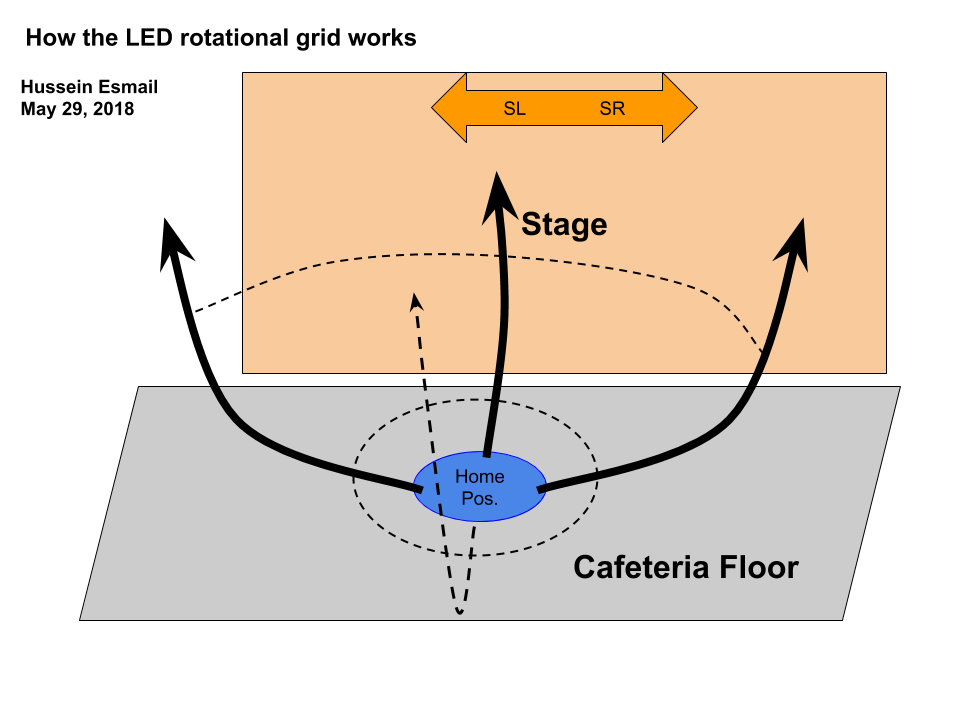
\includegraphics[width=\textwidth, keepaspectratio]{LED_Rotational_Grid.png}
    \end{center}
    \item \textbf{Intensity window}: This window is for the brightness of the LEDs. It has 3 rows, and is a fairly small window. The first row will consist of a button that is white and says ``Shutter open'' or blank that says ``Shutter closed''. The next two rows will say ``Strobe'' and ``Intensity''.
    \item \textbf{Beam window}: To clarify,``Beam'' refers to the focus/zoom of the light. If it hasa low zoom number, the light will be very wide and not as intense in one area, but more a general intensity. If it has a high zoom number, it is very focused, to roughly $1m^2$. This has only one slider on the window,and the size of the window is fairly similar to the brightness window.
    \item \textbf{Colors window}: Here is where the colours of the LEDs can be altered. There are a few options to changing colour.
    \begin{center}
        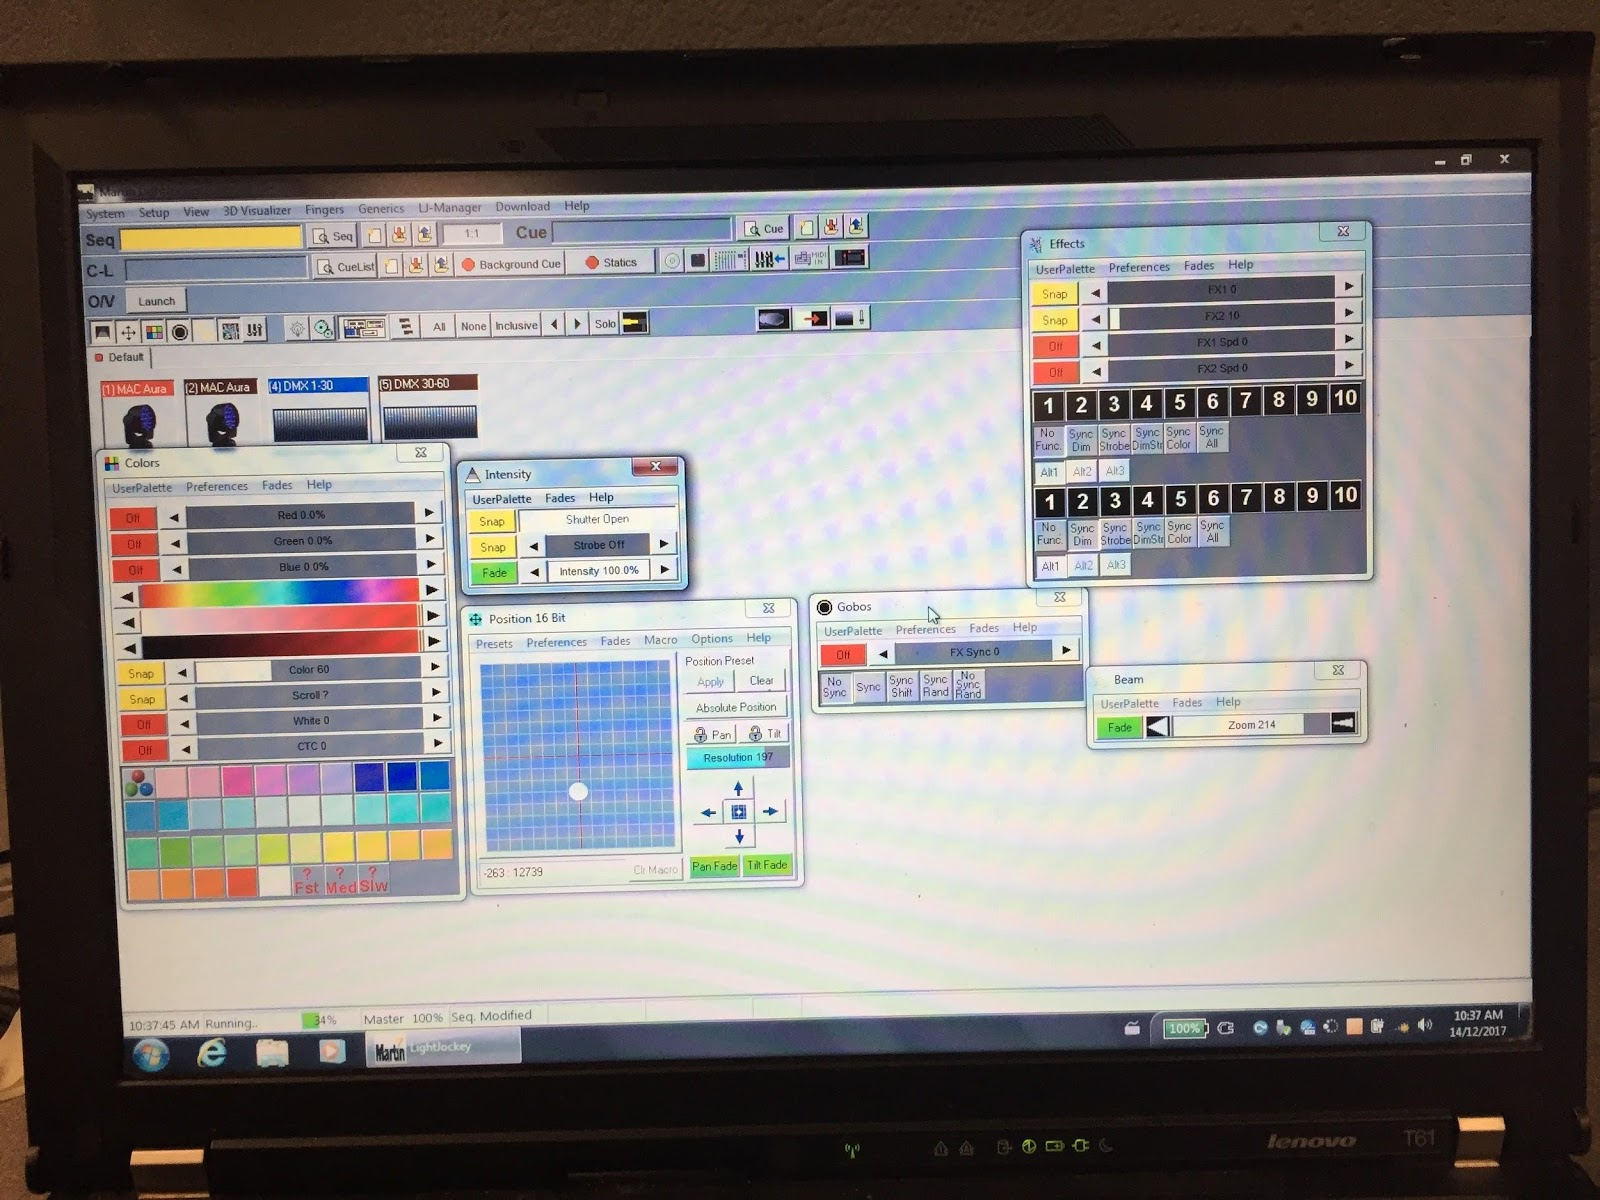
\includegraphics[width=\textwidth, keepaspectratio]{LightJockey_Screenshot.jpg}
    \end{center}
    \begin{enumerate}
        \item The first is the top 3 sliders which can alter the RGB (Red Green Blue) values and show them as percentages.
        \item The 4th to 6th slider which show the visual colours. I do not recommend using this as a main source of changing the colours, because this is dependent to the computer monitor’s colour scale for which colours you see on the screen. The first slider of this section is to alter the colour,the second is for the white levels,and the third the blacks.
        \item The 7th to 10th (4 sliders) are in general. See the list for more info.
        \begin{enumerate}
            \item Row 7: Colour slider, similar to the 4th slider showing the colour spectrum, but this time returns a numerical value,the maximum being 255.
            \item Row 8: This is the Scroll slider, which is used for displaying random colours at a certain speed. The slider controls how fast the randomization is.
            \item Row 9: This is the White levels, similar to row 5.
            \item Row 10: This is the CTC slider. To be honest, I have no idea what this means. The only use I have gotten out of this slider, is if you want a good shade of red, choose the 4th box on the 4throw of the preset boxes below (which will be discussed upon in point \underline{\ref{itm:colour_presets}}.) and set the CTC to 255(100\%). There is no other case where you would need this, so I recommend leaving it at 0 in any other case (unless I’m wrong$\ldots$).
        \end{enumerate}
        \item \label{itm:colour_presets} The boxes at the very bottom are preset colours you can click, and the LEDs will immediately go to that colour. I don’t know if these presets will change overtime, so I’ll refer to them as they are at the moment(see snapshot included). The first row of these are mainly pinks, purples, and dark blues. The second is an unnecessary number of shades of light blues. The third are greens and yellows,while the last are the reds along with a regular white(the white level will need to be at full to actually get a proper white). At the moment, I have no idea what the1st box on the 1st row does, nor the last 3 boxes on the last row. This would be a good subject of investigation for future students learning to operate this lighting.
    \end{enumerate}
    \item \textbf{Gobos window}: At the moment, I have no idea what this does, but there has not been a need for it so far, so this is another good topic of investigation.
    \item \textbf{Effects window}: Another irrelevant window because you have to set your own effects, but at the moment, there are none. Wow look at that! Another good investigation topic!
\end{enumerate}

\subsection{Lights in the Drama Room}
In the Drama room, there are more updated lights where each light takes up 6 channels each.The respective channels are as follows:
\begin{enumerate}
    \item Intensity
    \item Red
    \item Green
    \item Blue
    \item Lime (similar to yellow, but not quite)
    \item Strobe (I recommend not using this$\ldots$)
\end{enumerate}
On the \href{https://hussein-esmail7.github.io/site/lighting/downloads.html}{\underline{Downloads}} page of the \href{https://hussein-esmail7.github.io/site/lighting/index.html}{\underline{Lighting and Sound Manual Website}}, there is also a \href{https://hussein-esmail7.github.io/site/lighting/documents/Stage_lights_map.pdf}{\underline{map}} of where the lights are located to what lighting channels.

\subsubsection{Submaster Page for the Drama Room}
To make it easier for the Drama teachers, I made a submaster page on the lighting board that turns on specific areas with specific colours. This page is located on Submaster Page 1. If for whatever reason it’s not there anymore, I have also uploaded the document with all the lighting numbers that were on each submaster. \href{https://hussein-esmail7.github.io/site/lighting/documents/Drama_room_submasters.docx}{\underline{You can find it here}}.

\section{Lights in Other Theatres}
\subsection{What boards other locations have}
\begin{itemize}
    \item \href{https://oshawalittletheatre.com}{\textbf{\underline{Oshawa Little Theatre (OLT) (62 Russett Ave, Oshawa,ON L1G 3R5)}}}: ITC Element (60 channel) Lighting Board
    \item \href{https://www.aultsvilletheatre.com/}{\textbf{\underline{Aultsville Theatre, Cornwall, Ontario}}}: Canto 1200msd/msr MK2 Spotlight, lighting board unknown. Spotlight is roughly 10m away from the lighting board, and may require an additional operator if there isn't enough time to go between the two machines.
    \item \textbf{J. Clarke Richardson Collegiate(1355 Harwood Ave N, Ajax, ONL1T 4G8)}: The lights at this school are as follows in the diagram. Each circle represents one light where they are positioned as of March 1,2018. In downstage right, there is absolutely no light, so it is recommended that you alter planned blocking accordingly before the tech set up day.
    \begin{center}
        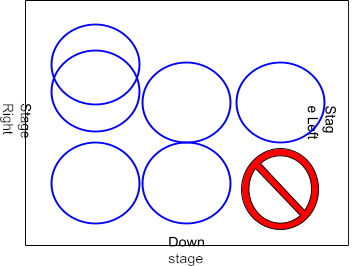
\includegraphics[height=2in, width=\textwidth, keepaspectratio]{Richardson_Lighting.png}
    \end{center}
\end{itemize}

At other theatres, they use more updated boards, which almost always include the use of monitors (sometimes more than one).

\section{Sound}
\subsection{Sound board in the Lighting Booth}
To power up the sound system in the lighting booth,you first need to power on the soundboard. You do this by pressing a small black button on the back of the board slightly to the right from the middle. After you have confirmed that the board is on, you can now turn on the Carver
Pro Xi2600 speaker system that is backstage on Stage Right, on the side closer to the hallway. To do that, there are a few steps:
\begin{enumerate}
    \item There are 3 power switches:
    \begin{enumerate}
        \item The top right corner, there is a push button
        \item The left side, there is a switch
        \item And finally, the bottom right switch
    \end{enumerate}
    \item There are 2 circular dials in the lower left side of the console. Make sure that both of them are facing 3 o’clock.
\end{enumerate}
The systems are now ready to perform audio tasks.

Please note: When plugging in/removing a microphone from a channel, make sure that the respective channel is muted, or else there will bea power surge, which can be identified by aloud “pop” sound on the speakers (and annoyed reactions from the audience/anyone in the cafeteria)

When turning off the speaker and sound board, the speaker must be turned off first, or else there will be a power surge (see note above). To turn off the speaker, do the following. These don’t need to be done in any particular order.
\begin{enumerate}
    \item There are 3 power switches:
    \begin{enumerate}
        \item The top right corner, there is a push button
        \item The left side, there is a switch
        \item And finally, the bottom right switch
    \end{enumerate}
    \item There are 2 circular dials in the lower left side of the console. Make sure that both of them are to the left as much as possible.
\end{enumerate}

To turn off the sound board, first make sure all channels are muted. Then, on the very right side of the board, make sure the Center, Left, and Right faders are all off. Then press the power button on the back of the board.

\subsection{Playing music from an external device to the Cafeteria sound system}

To play music from an external device, you would need the proper wire that converts AUX toXLR or $1/4$” stereo. But luckily, the way the projector sound goes to the sound board, is that it is run through an Ethernet cable, then converted by AUX(in the converter), to ¼” stereo. What that means is that you can unplug it straight from the converter (the tiny converter calledKramer Tools XGA/Audio Line Receiver TP-122) and use the AUX directly from your device.

Please note, that if this is unplugged, the projector sound will not work, because it is originally run through this cord as well.

For playing video to the projector from the booth, please see \textbf{\underline{\ref{sec:caf_projector}}}.

\subsection{Sound in the Gym}
Before setting up the sound system in the gym, make sure you acquire the proper components that are not already there (microphones, extension cords for the portable sound system, and as many XLR 3-pin cords you can find, trust me, they’ll feel short in the gym). Make sure you also check with the Comtech Room (Room 120) and the MusicRoom for any extra XLR cords.

To play sound in the \textbf{large} gym, there is a portable sound system in the equipment room (the one located more to the right). Once you have gotten that, connect the speaker output to theXLR input in the wall located in the left corner of the gym, near the door to the small gym.While doing this, make sure the power to the speakers in the gym are off, to ensure that there will be no power surges.

Sound in the gym is mainly used to host the JuniorAwards ceremony and the Commencement ceremony for the grade 12s who have already graduated.While setting up for these two, please be courteous to the custodians if they are setting up chairs and/or the black platform that the principal/vice principals will be standing on to handout the certificates.

\subsection{Sound in the Library}
In the library, all the sound-related systems are stored in a small black cabinet near the SeminarB entrance, and all handheld devices (microphones,computer wires, etc.) are stored in the cabinet of the cart on wheels.

In the black cabinet, the amp is at the very bottom (model of the amp: TOA Mixer AmplifierBG-235). Make sure not to change any of the volume knobs because they are already set by Ms.Hung. On the higher shelf, you’ll find the microphone receiver. It is a TOA Diversity WirelessTuner WT-4820, which has 2 microphone inputs. In the cart cabinet, there’s only one microphone, so it’s possible that Ms. Hung has another one somewhere in the library.

\subsection{Sound in other theatres}
If you are playing sound in other theatres/schools, make sure that you follow instructions given by the supervisor from that school (there isn’t much info in this section, basically don’t do anything stupid).

\subsection{Intercom Systems}
In full-scale theatres, there are also intercom systems so that people don’t have to be too loud when talking to people. They can simply talk into their own microphone and the people also wearing those headsets will hear them. Since this is not broadcasted on the speaker system, the sound board is not needed (meaning it works even if the sound board is off).

\begin{center}
    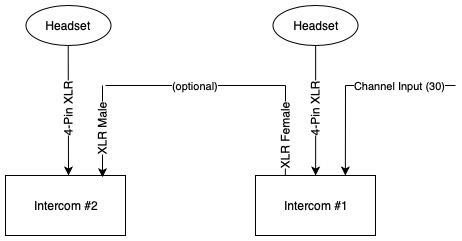
\includegraphics[width=\textwidth, keepaspectratio]{Intercom_Wiring.jpg}
\end{center}

\subsubsection{Connecting the Intercom}
On the back of the intercom receiver, are 3 ports (1 XLRMale, 1 4-Pin XLR Male, and an XLR Female). The input for the channel goes into the male XLR input (the wire should be XLR female). The headset goes in the middle port, which is the 4-Pin XLR. The last port is for output which is not necessary. When connecting intercoms,they don’t all need to be connected directly to the channel. By this I mean an intercom can be connected to another intercom which is connected to the channel. This would be ideal for use in the lighting booth, so that the lighting technician and sound technician each get an intercom.

\subsubsection{Where to find the intercom inputs}
The wire to plug it in is Channel 30 as an XLR.
\begin{itemize}
    \item Booth input: The booth input is simply a wire, which connects to the intercom receiver directly. It should be labeled ``INTERCOM'' on masking tape or ``30'' (because of the channel number).
    \item Backstage input: This input is at the bottom of the speaker system, on the left side.
    \item Drama Room input: When you walk into the Drama Room, the port is in the middle of the wall that the entrance door is also on.
\end{itemize}

\section{Other}
\subsection{Cafeteria Projector} \label{sec:caf_projector}
To play video from the booth to the projector in the cafeteria, you must have a device that can connect to a VGA video output.

In the booth, the video normally comes from the stage through Ethernet, then to the KramerPresentation Switcher Scaler HQV VP-728 then to theMagenta console (which had a ``Video to Projector'' label on it), then goes back out the wall through Ethernet to the Projector. The audio comes from the wall directly into the ``Video to Projector'' console. This is how it normally should be for the projector input by the speaker to work.

To play video from the booth, you need to take the input cord from the Kramer Presentation Switcher/Scaler HQV VP-728 and put another VGA cord from the computer into it.

\textbf{Please note}: You must put these cords back the proper way to ensure the functionality of the stage video input

\textbf{Future improvement}: In the future, it might be possible to have just one system that goes like this: Input from downstairs to [unnamed console] to Projector, where the audio would also go into the [unnamed console].

\subsection{Library Projectors}
In the library, there are 2 projectors, both on the wall with the windows to the catwalk. You can either use each one for one computer or show the same thing on both screens. To turn on the projectors, there are 2 separate power switches. The one closer to the Seminar B entrance is actually right beside the Seminar B entrance door.The power switch of the projector closer to the library entrance is near where the fireplace is.

If you want both projectors to show the same thing, you must make sure you do the following:
\begin{enumerate}
    \item The computer is plugged into the projector closest to the library entrance. If you need a longer VGA wire, there is one in the cart cabinet. Also feel free to move the cart near the fireplace to reach the input.
    \item On the projector closest to Seminar B, the input is set to ``PC''.
    \item On the projector closest to the main entrance, the input is set to ``Computer 2''. If it was ``Computer 1'', make sure to put it back to that when you’re done.
\end{enumerate}

If you want to transmit audio from the computer to the speakers, you have to use the AUX cordon the VGA cable. If you want to change the volume of the sound, the only places you can change it are on the computer, or the projector switch by the fireplace.

\subsection{Links for Further Reading}
\begin{itemize}
    \item For instruction manuals for any of the Strand Lighting products, you can visit \href{http://www.strandlighting.com/support-documents/}{\underline{this site}} and specify the model.
    \item Martin LightJockey 1.0 Software Manual \href{http://www.martin.com/files/files/productdocuments/11_MANUALS/999/UM_LJ_EN_d.pdf}{\underline{can be accessed here}}.
    \item Setting Submasters for ETC lighting consoles can be found at  \href{https://www.reddit.com/r/techtheatre/comments/7qsf7d/etc_express_programming/?st=JCXGJGZI&sh=654a9e9b}{\underline{this Reddit post}}.
\end{itemize}

\section{Video Tutorials for Lighting}
\begin{itemize}
    \item Setting Submasters for the Strand 200 Lighting board can be found \href{https://m.youtube.com/watch?v=PftZWxb1ETA}{\underline{here}}.
    \item Making proper lighting charts with Submasters can be found \href{https://m.youtube.com/watch?v=jzFnM5nUZvY}{\underline{here}}.
\end{itemize}

\end{document} % Official end of the document. 
